\chapter{Schematic}


\section{Altium tutorial}


See the ENCE461 Learn page for the Altium tutorial.


\section{Suggestions}

\begin{enumerate}
\item If you get the schematic wrong, the PCB will be wrong, and you
  will have rework grief (see \hyperref[rework]{rework}).

\item A clear schematic is important for debugging.

\item In general, you should aim to have inputs on the left, outputs
  on the right, higher voltages at the top.

\item Add notes to explain anything non-obvious.
\end{enumerate}



\section{Check list}
\label{schematic-check-list}

You must check the schematic carefully.  I use a highlighter to mark
every wire and component.  If you get the schematic wrong, the PCB
will be wrong, and you will have to do much rework, see
\reffig{rework}.


\begin{figure}[!h]
  \centering
  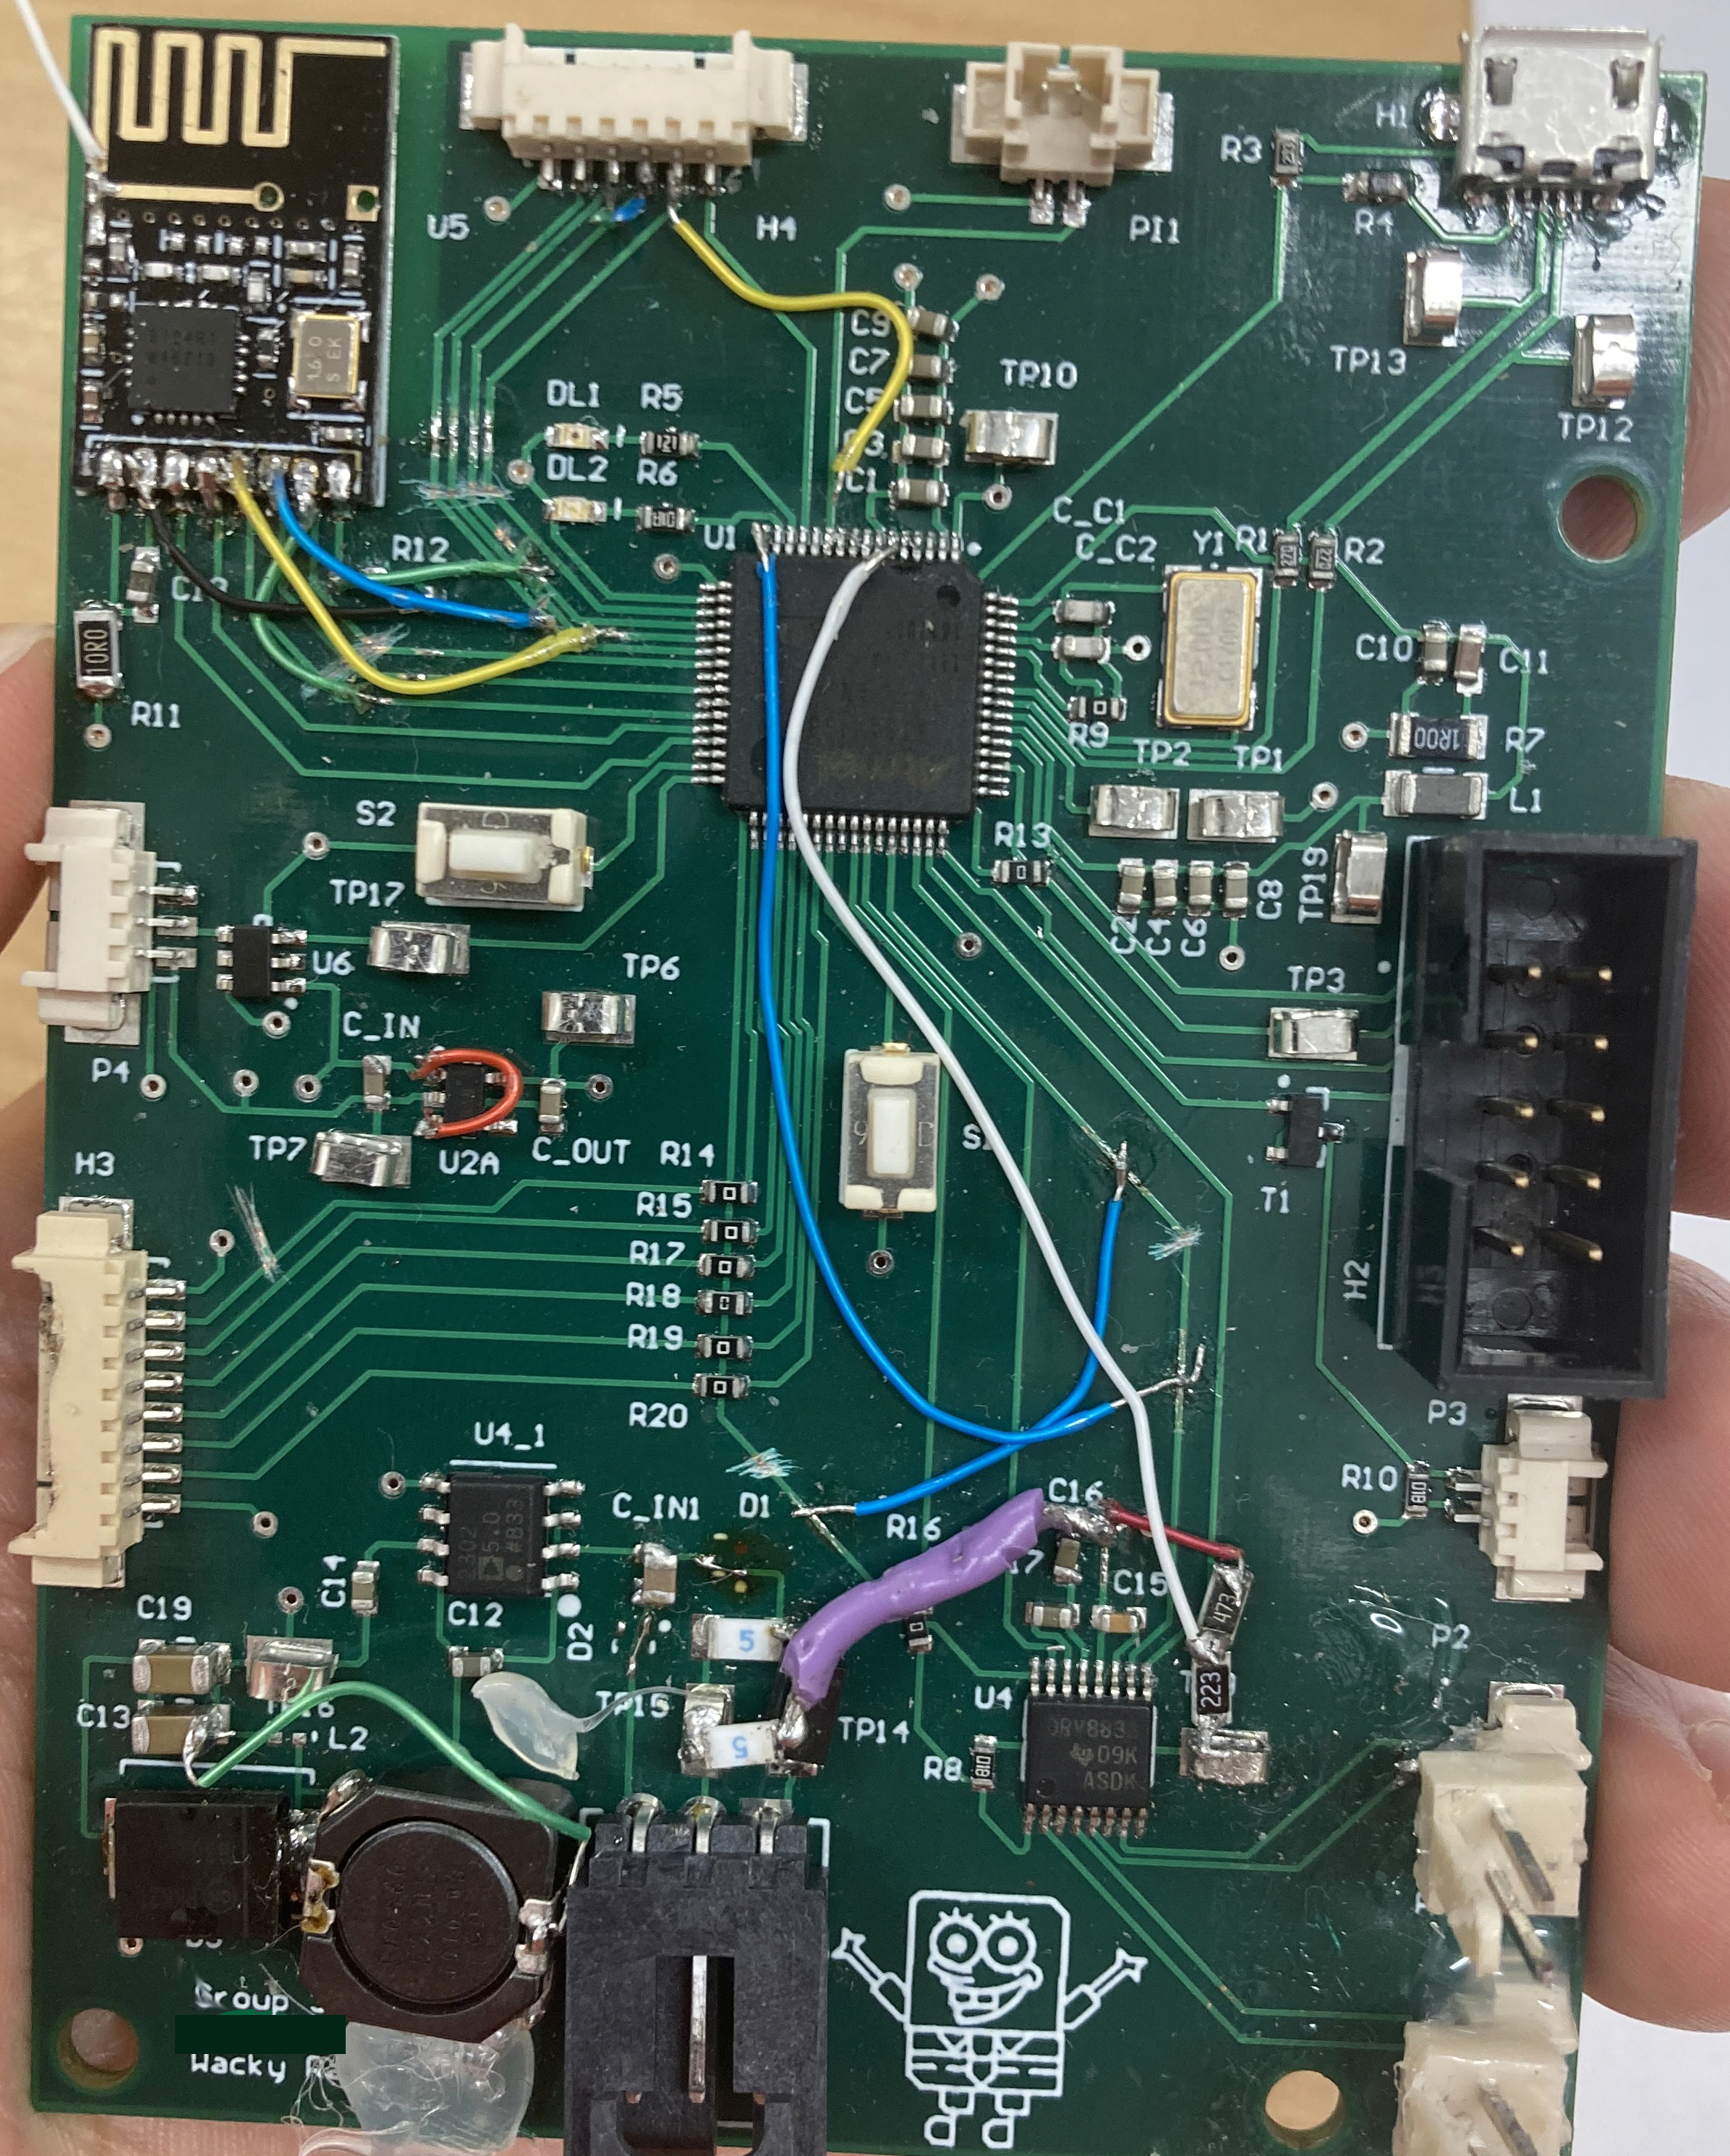
\includegraphics[width=6in]{figs/rework.jpg}
  \caption{Example of a PCB where not much care was taken with the
    schematic resulting in a lot of rework.  And yes, the board worked
    in the end.}
  \label{fig:rework}
\end{figure}



\begin{enumerate}
\item
  The SPI signals for the radio are connected to the correct MCU pins.
\item
  The PWM signals for the motor are connected to the correct MCU pins.
  Note, the PWMLx and PWMHx pins are complementary and cannot be driven
  independently.
\item
  All the MCU VDD pins need to be powered.
\item
  All the MCU GND pins need to be connected to ground.
\item
  Avoid connecting to \pin{PB4} and \pin{PB5} (say for TWI1).  If you
  do you will need to disable JTAG in software.
\end{enumerate}
